\documentclass[11pt]{article}

\usepackage[margin=1in]{geometry}
\usepackage{amsfonts, amsmath, amssymb}
\usepackage[none]{hyphenat}
\usepackage{fancyhdr}
\usepackage{graphicx}
\usepackage{float}
\usepackage[nottoc, notlot, notlof]{tocbibind}
\usepackage{hyperref}
\usepackage[french]{babel}

\pagestyle{fancy}
\fancyhead{}
\fancyfoot{}
%\fancyhead[L]{\slshape \MakeUppercase{Radio}}
\fancyhead[R]{\slshape Projet Réseaux}
\fancyfoot[C]{\thepage}
\renewcommand{\footrulewidth}{0pt}

\parindent 0ex %
\renewcommand{\baselinestretch}{1.5}

\begin{document}

\begin{titlepage}
\begin{center}
\vspace*{1cm}
\Large{\textbf{Projet Réseaux}}\\
\vfill
\line(1,0){400}\\[1mm]
\huge{\textbf{Simulation d'un protocole de routage à vecteur de distances}}\\[3mm]
\Large{\textbf{- Rapport, groupe 2 -}}\\[1mm]
\line(1,0){400}\\
\vfill
Abdelkrim ESSAFSYFY, matricule : 191856\\
Paul ONDAFE MATOCK, matricule : 202048\\
Année académique 2020-2021
\end{center}
\end{titlepage}

\tableofcontents
\thispagestyle{empty}
\clearpage
\setcounter{page}{1}

\section{Exercice 2.2}
\begin{figure} [h!]
\centering
  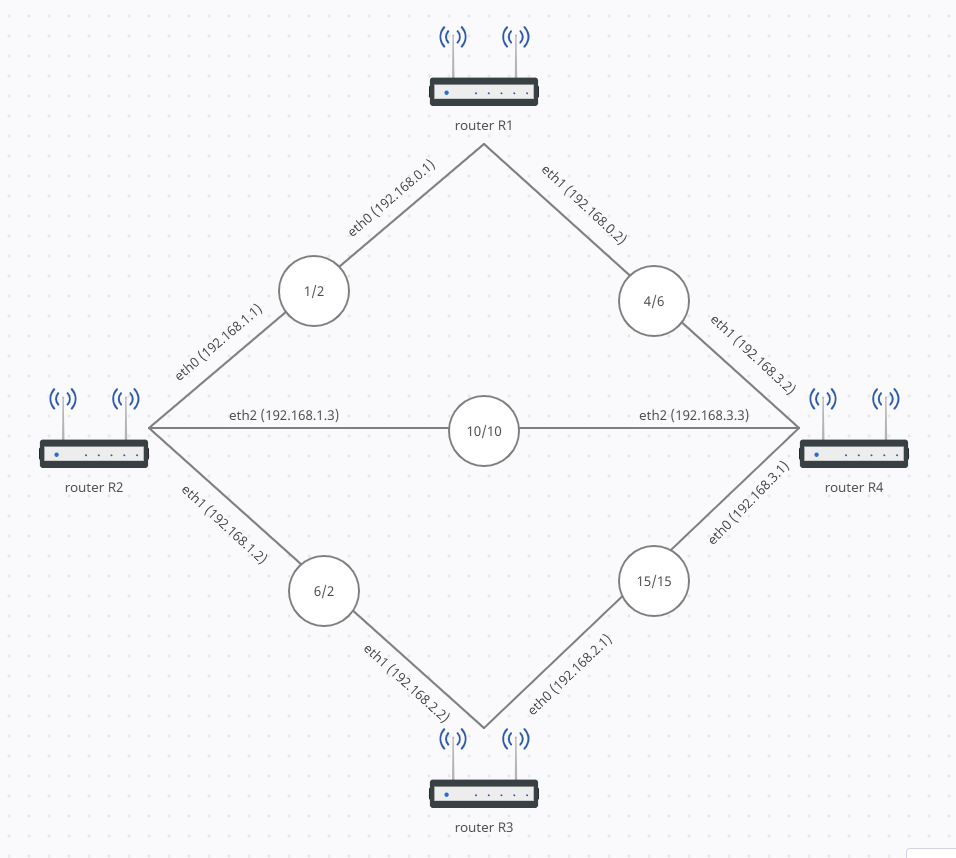
\includegraphics[width=0.65\textwidth]{../documents/topology-figure.png}
  \caption{Topologie de 4 nœuds et 5 liens}
   \label{fig:topology}
\end{figure}
\begin{figure} [h!]
\centering
  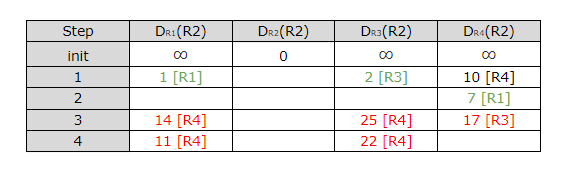
\includegraphics[width=0.65\textwidth]{../documents/demo-table.png}
  \caption{Tableau des routes calculées par les routeurs vers R2}
   \label{fig:table}
\end{figure}

La Figure \ref{fig:topology} représente une topologie contenant 4 nœuds et 5 liens ainsi que les coûts et les interfaces par lesquelles ils sont connectés. La figure \ref{fig:table} quant à elle, représente les routes calculées à partir de chacun des routeurs vers une unique destination \textit{(R2)}.



\section{Exercice 2.3}
\begin{figure} [h!]
\centering
  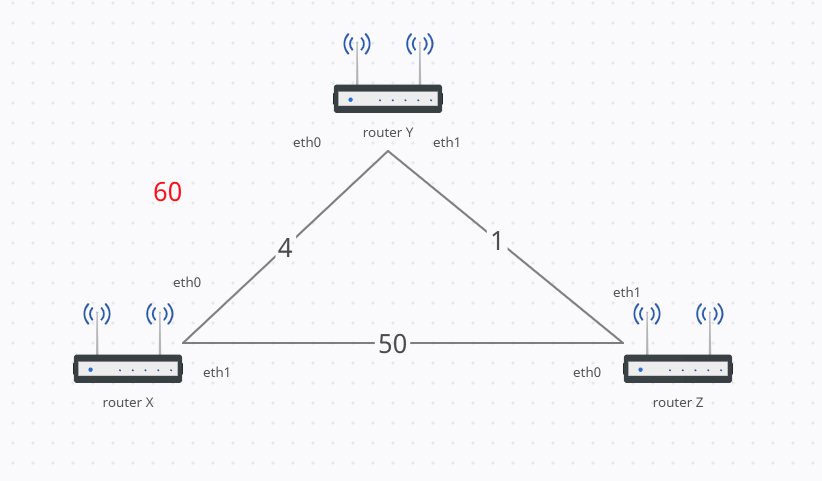
\includegraphics[width=0.65\textwidth]{../documents/infinity-figure.png}
  \caption{Topologie résultant en un comptage à l'infini}
   \label{fig:inf-topo}
\end{figure}
\begin{figure} [h!]
\centering
  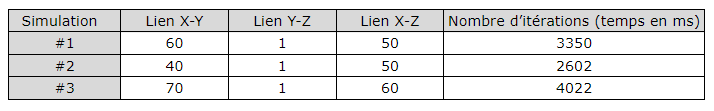
\includegraphics[width=0.65\textwidth]{../documents/infinity-table.png}
  \caption{Tableau contenant 3 simulations différentes}
   \label{fig:inf-table}
\end{figure}

La Figure \ref{fig:inf-topo} représente la topologie résultant en un comptage à l'infini, le nombre 60 en rouge indique le changement nécessaire pour provoquer le comptage à l'infini.\\

Le nombre de messages échangés par les routeurs depuis le changement de métrique et jusqu'à la nouvelle convergence est de 24 messages.\\

Les 2 assignations de coûts de liens qui résultant en une convergence plus courte et une autre plus longue sont renseignées dans la Figure \ref{fig:inf-table}.



\section{Exercice 2.4}
La nom de la solution au comptage à l'infini vue dans le cours est \textit{Poisoned reverse}. Elle consiste à ne pas indiquer le coût réel vers la destination aux voisins (en leur envoyant $+\infty$ comme coût) qui passent par ce même nœud afin d'éviter de progressivement incrémenter de 1 les coûts. Dans la topologie donnée dans l'exercice 2.3, $Y$ doit renseigner $+\infty$ à $Z$ --- son voisin --- puisque celui-ci passe pas $Y$ afin d'atteindre $X$ ; sa destination.\\



\section{Exercice 2.5}
\begin{figure} [h!]
\centering
  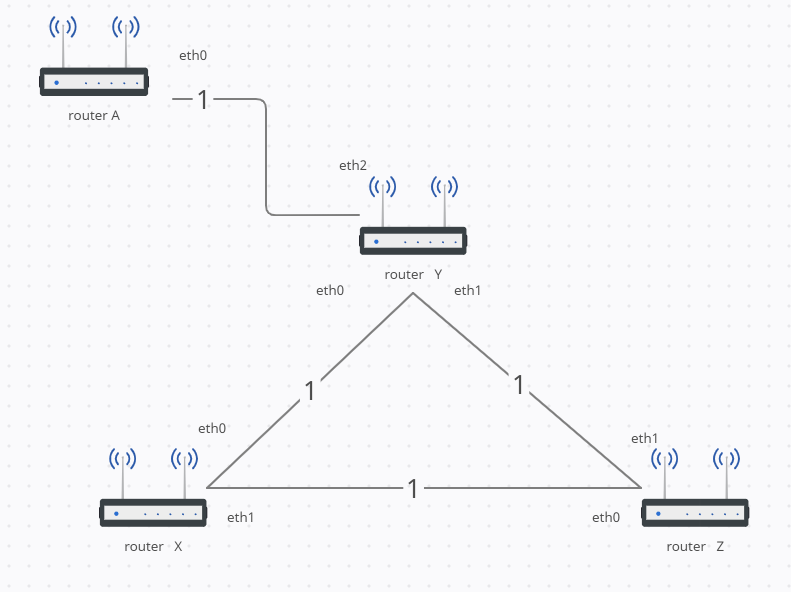
\includegraphics[width=0.65\textwidth]{../documents/problem-figure.png}
  \caption{Topologie où Poisoned reverse ne règle pas le problème de comptage à l'infini}
   \label{fig:prob-topology}
\end{figure}

La Figure \ref{fig:prob-topology} contient une topologie où, même avec application de la méthode Poison reverse, le problème de comptage à l'infini persiste. Dans cette topologie, le lien entre le routeur $A$ et le routeur $Y$ n'est plus fonctionnel. Il est donc impossible d'accéder au routeur $A$.\\

\subsection{Persistance du problème de comptage à l'infini}
Le problème de comptage à l'infini persiste car, malgré le fait que le routeur $Y$ informe $X$ et $Z$ que le coût vers $A$ est égal à l'infini, le premier routeur recevant cette information --- supposons dans ce cas qu'il s'agit de $Z$ --- remarque qu'il est toujours possible d'accéder au routeur $A$ via $X$. Ceci est dû au fait que $X$ n'est pas au courant du changement des coûts des liens ($D_{y}(a)=+\infty$). Nous remarquerons donc un comptage à l'infini entre $X$ et $Z$, qui continuent d'incrémenter les coûts.\\

\subsection{Solution au comptage à l'infini}
Une solution à ce problème est appelée \textit{Split Horizon}. Elle consiste à interdire à un routeur de partager les coûts des liens dans la table de routage avec le routeur (interface) à partir duquel il a appris ceux-ci. Concrètement, dans la Figure \ref{fig:prob-topology}, quand le routeur $Y$ informe $Z$ --- et plus tard $X$ --- que le routeur $A$ n'est plus accessible, le routeur $Z$ n'enverra pas à $Y$ les coûts associés à ce routeur $Y$. De cette façon, $Y$ conservera $D_{y}(a)=+\infty$ et le comptage à l'infini sera évité.



\section{Exercice 2.6}
\begin{figure} [h!]
\centering
  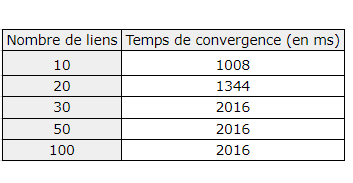
\includegraphics[width=0.45\textwidth]{../documents/convergence-graphs.png}
  \caption{Tableau de convergence avec différents liens}
   \label{fig:graphs}
\end{figure}
La Figure \ref{fig:graphs} représente le temps convergence obtenus pour des topologies de 10, 20, 30, 50 et 100 liens.
\vspace{10px}

\subsection{Fonctionnement de l'algorithme}
Le principe utilisé se décline de la manière suivante : création des différents nœuds qui seront utilisés dans le réseau. En suite, initialisation du réseau par deux nœuds avec un lien. Finalement, ajout d’un nœud dans le réseau existant en s’appuyant sur le model de Barabási, le choix de rattacher le nouveau nœud à un des nœuds du réseau selon le degré de ce dernier. On réalise une itération sur ce point tout vérifiant que la condition de la densité est toujours respectée.\\

\subsection{Description du lancement du programme}
L'algorithme a été conçu en Java. Le package contient quatre classes. La classe Main.java, qui permet de lancer la simulation, une classe Node.java qui simule un noeud (notamment un routeur), une classe Link.java qui elle simule un lien entre deux noeuds (ou, encore une fois, deux routeurs) et finalement une classe Generator.java qui crée la topographie et la stocke dans un fichier texte nommé 'graph.txt'. 

\topskip0pt
\vspace*{\fill}

\end{document}